% sections/evaluation.tex

\section{Evaluation}
\label{sec:evaluation}

We evaluate the routing system across three dimensions: signal extraction efficiency, LoRA multi-task scaling, and end-to-end routing correctness.

\subsection{Signal Extraction Latency}

\Cref{tab:signal_latency} reports median and p99 latencies for each signal type on an NVIDIA A100 GPU with ModernBERT base model.

\begin{table}[h]
\centering
\caption{Signal extraction latency by type}
\label{tab:signal_latency}
\begin{tabular}{lrrl}
\toprule
\textbf{Signal Type} & \textbf{Median} & \textbf{p99} & \textbf{Requires ML} \\
\midrule
Keyword      & $< 0.1$\,ms & $< 0.5$\,ms  & No \\
Context      & $< 0.1$\,ms & $< 0.5$\,ms  & No \\
Language     & $< 0.5$\,ms & $< 1$\,ms    & No \\
Authorization & $< 0.1$\,ms & $< 0.5$\,ms & No \\
\midrule
Embedding    & $15$\,ms    & $45$\,ms     & Yes \\
Domain       & $60$\,ms    & $120$\,ms    & Yes \\
Fact-check   & $55$\,ms    & $110$\,ms    & Yes \\
Modality     & $50$\,ms    & $100$\,ms    & Yes \\
Feedback     & $55$\,ms    & $115$\,ms    & Yes \\
Complexity   & $50$\,ms    & $105$\,ms    & Yes \\
Preference   & $55$\,ms    & $110$\,ms    & Yes \\
\bottomrule
\end{tabular}
\end{table}

Heuristic signals complete in sub-millisecond time, while ML signals range from 15--120\,ms.
With parallel evaluation, the wall-clock time is dominated by the slowest active signal ($\sim$120\,ms for domain classification) rather than the sum.

\subsection{LoRA Memory Efficiency}

\Cref{tab:lora_memory} shows the memory advantage of serving classifiers via LoRA adapters versus independent fine-tuned models.

\begin{table}[h]
\centering
\caption{Model memory: independent fine-tuned models vs.\ LoRA adapters (ModernBERT base, 150M params)}
\label{tab:lora_memory}
\begin{tabular}{lrr}
\toprule
\textbf{Tasks ($n$)} & \textbf{Independent (MB)} & \textbf{LoRA (MB)} \\
\midrule
1 & 573   & 573 \\
3 & 1{,}719 & 574 \\
6 & 3{,}438 & 575 \\
\bottomrule
\end{tabular}
\end{table}

At $n = 6$, the LoRA architecture requires $\sim$6$\times$ less model memory (one base model + six $\sim$0.2\,MB adapters vs.\ six full model copies).
Each task still requires its own forward pass; latency reduction comes from \emph{parallel execution} of classifiers rather than from LoRA itself (\Cref{sec:lora_mom}).

\subsection{Decision Engine Overhead}

Decision evaluation adds negligible latency:
$< 0.1$\,ms for 10 decisions with 3 conditions each;
$< 0.5$\,ms for 100 decisions with 5 conditions each.
This confirms that the $O(M \cdot L_\text{max})$ complexity is dominated by signal extraction.

\subsection{Composable Orchestration Across Deployment Scenarios}

A key claim of this work is that the same architecture serves diverse deployment scenarios through configuration.
\Cref{tab:deployment_scenarios} demonstrates how different signal-decision-plugin compositions address different requirements:

\begin{table}[h]
\centering
\caption{Composable signal orchestration across deployment scenarios. Each scenario activates a different subset of the eleven signal types, selection algorithms, and plugin chains---using the same system binary and architecture.}
\label{tab:deployment_scenarios}
\begin{tabular}{p{2.5cm}p{3cm}p{2.5cm}p{3.5cm}}
\toprule
\textbf{Scenario} & \textbf{Active Signals} & \textbf{Selection} & \textbf{Key Plugins} \\
\midrule
Privacy-regulated (healthcare) & authz, domain, language & Static (compliant models only) & Strict PII redaction, no caching, audit logging \\
Cost-optimized (developer tool) & complexity, embedding, keyword & AutoMix cascade & Aggressive semantic cache, header mutation for LoRA adapter \\
Multi-cloud enterprise & domain, modality, authz & Latency-aware & Multi-endpoint failover, provider auth factory, system prompt injection \\
Multi-turn assistant & embedding, feedback, preference & Elo with session pin & Responses API state, memory retrieval, RAG injection \\
\bottomrule
\end{tabular}
\end{table}

\subsection{End-to-End Routing Correctness}

The end-to-end test framework validates routing behavior across eight scenario profiles:

\begin{table}[h]
\centering
\caption{End-to-end test profiles}
\label{tab:e2e_profiles}
\begin{tabular}{lp{8cm}}
\toprule
\textbf{Profile} & \textbf{Validated Behavior} \\
\midrule
Multi-endpoint      & Multi-provider routing with weighted distribution and failover across heterogeneous backends \\
Multi-provider auth & Provider-specific auth injection (API key, OAuth2, cloud IAM) via authorization factory \\
AuthZ-RBAC          & Role-based model access (admin/premium/free tiers) with authz signal \\
ML model selection  & KNN, KMeans, SVM, MLP selection accuracy on held-out queries \\
Keyword routing     & Keyword signal matching with AND/OR/NOR combinators \\
Embedding routing   & Embedding similarity thresholds and confidence-based decision selection \\
RAG + Responses API & Context retrieval, injection, and stateful multi-turn via Responses API \\
Routing strategies  & Static, Elo, RouterDC, AutoMix, Hybrid algorithm comparison \\
\bottomrule
\end{tabular}
\end{table}

Each profile validates correct model selection, safety enforcement (jailbreak blocked, PII detected), cache behavior (hits after similar queries), multi-provider routing (correct endpoint resolution and auth injection), and header propagation.

\subsection{Semantic Cache Effectiveness}

At a similarity threshold $\theta = 0.92$:
exact-match queries achieve 100\% hit rate with $< 5$\,ms lookup latency;
paraphrased queries achieve 60--80\% hit rate depending on paraphrase distance.
Cache hits eliminate backend model invocation entirely, reducing per-request cost to embedding computation only.

\subsection{Unified MoM Evaluation Framework}

To validate the robustness of the Mixture of Models (MoM) collection, we implemented a unified evaluation pipeline that benchmarks both merged models and LoRA adapters. The framework standardizes the assessment of heterogeneous model variants across intent classification and PII detection tasks.

The evaluation architecture, shown in \Cref{fig:eval_pipeline}, utilizes the following components:

\begin{itemize}
    \item \textbf{Schema Normalization:} Inputs from diverse sources—including MMLU-Pro for intent and Presidio for token classification—are mapped to a common evaluation schema.
    \item \textbf{Comparative Quality Validation:} The system computes weighted F1-scores and per-class precision/recall to ensure that the memory efficiency gains reported in \Cref{tab:lora_memory} do not result in significant predictive degradation compared to full-parameter models.
    \item \textbf{Parallelized Benchmarking:} Large-scale evaluations are executed via \texttt{ProcessPoolExecutor} to minimize wall-clock time. The pipeline incorporates automated OOM recovery and exponential backoff for API-based signal providers to ensure benchmark reliability.
\end{itemize}

Results include p50 and p99 latency profiling to confirm that model orchestration remains within the operational bounds required for real-time routing.

\begin{figure}[ht]
    \centering
    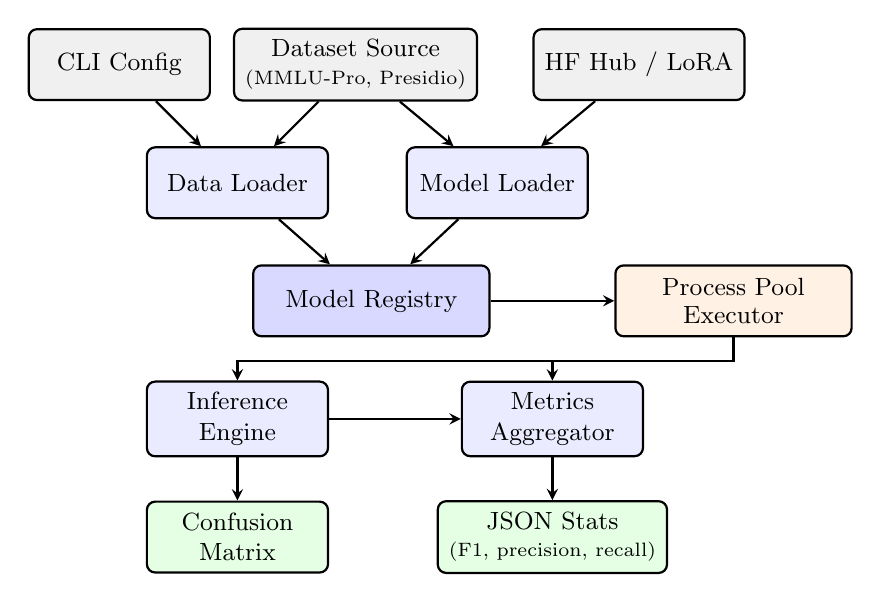
\begin{tikzpicture}[
      box/.style={rectangle, draw, thick, rounded corners=3pt,
                  minimum height=0.9cm, minimum width=2.3cm,
                  align=center, inner sep=4pt, font=\small},
      src/.style={box, fill=gray!12},
      proc/.style={box, fill=blue!8},
      outbox/.style={box, fill=green!10},
      arr/.style={->, >=stealth, thick},
      lbl/.style={font=\scriptsize, midway, above},
    ]

    % Row 1: Config + Data sources
    \node[src] (cli) at (0, 3) {CLI Config};
    \node[src] (ds)  at (3, 3) {Dataset Source\\[-1pt]\scriptsize(MMLU-Pro, Presidio)};
    \node[src] (hf)  at (6.6, 3) {HF Hub / LoRA};

    % Row 2: Loaders
    \node[proc] (dl) at (1.5, 1.5) {Data Loader};
    \node[proc] (ml) at (4.8, 1.5) {Model Loader};

    % Row 3: Central engine
    \node[proc, fill=blue!15, minimum width=3cm] (reg) at (3.2, 0)
      {Model Registry};
    \node[proc, fill=orange!10, minimum width=3cm] (pool) at (7.8, 0)
      {Process Pool\\[-1pt]Executor};

    % Row 4: Inference + metrics
    \node[proc] (inf) at (1.5, -1.5) {Inference\\Engine};
    \node[proc] (agg) at (5.5, -1.5) {Metrics\\Aggregator};

    % Row 5: Outputs
    \node[outbox] (cm)   at (1.5, -3) {Confusion\\Matrix};
    \node[outbox] (json) at (5.5, -3) {JSON Stats\\[-1pt]\scriptsize(F1, precision, recall)};

    % Arrows: sources to loaders
    \draw[arr] (cli) -- (dl);
    \draw[arr] (ds)  -- (dl);
    \draw[arr] (ds)  -- (ml);
    \draw[arr] (hf)  -- (ml);

    % Arrows: loaders to registry
    \draw[arr] (dl) -- (reg);
    \draw[arr] (ml) -- (reg);

    % Arrow: registry to pool
    \draw[arr] (reg) -- (pool);

    % Arrows: pool to inference and metrics
    \draw[arr] (pool.south) -- ++(0,-0.3) -| (inf.north);
    \draw[arr] (pool.south) -- ++(0,-0.3) -| (agg.north);

    % Arrows: inference to outputs
    \draw[arr] (inf) -- (cm);
    \draw[arr] (inf.east) -- ++(0.4,0) |- (agg.west);
    \draw[arr] (agg) -- (json);

    \end{tikzpicture}
    \caption{Unified MoM evaluation pipeline. Configuration and dataset sources feed into the data and model loaders, which populate the model registry. A process pool executor parallelizes inference across model variants, producing confusion matrices and aggregated metrics (weighted F1, per-class precision/recall) for both merged and LoRA models.}
    \label{fig:eval_pipeline}
\end{figure}

\subsection{Open Evaluation}

Detailed model selection quality comparisons across algorithms, HaluGate detection accuracy on standard benchmarks (HaluEval, FActScore), and large-scale routing quality evaluation are under preparation in collaboration with the RouterArena team.

\paragraph{Contributors.}
Senan Zedan, Xunzhuo, yehudit1987, abdallahsamabd, Noa Limoy, Yossi Ovadia, Liav Weiss, Huamin Chen, samzong, Jintao Zhang, asaadbalum, Xunzhuo, Srinivas A, Marina Koushnir, Chever John, Chaojun Zhang, Avishek Goswami, Zohaib Hassnain.

